% Website copy (Research, Policy Analysis and Policy Maker circles all 2.4cm).
% Original: overleaf-new/assets/evidence-to-policy.tex
% Standalone TikZ source for the "Truth → Research → Policy Analysis →
% Policy Makers → Support/Oppose" diagram. Used in the Registration-Tips
% deck (About Me / Motivation for Evidence Aggregation slide).
%
% Build:
%   xelatex evidence-to-policy.tex     (or pdflatex)
%   pdftools::pdf_render_page(...) -> high-DPI PNG

\documentclass[border=10pt,tikz]{standalone}
\usepackage{tikz}
\usetikzlibrary{positioning,shapes.geometric}

\begin{document}
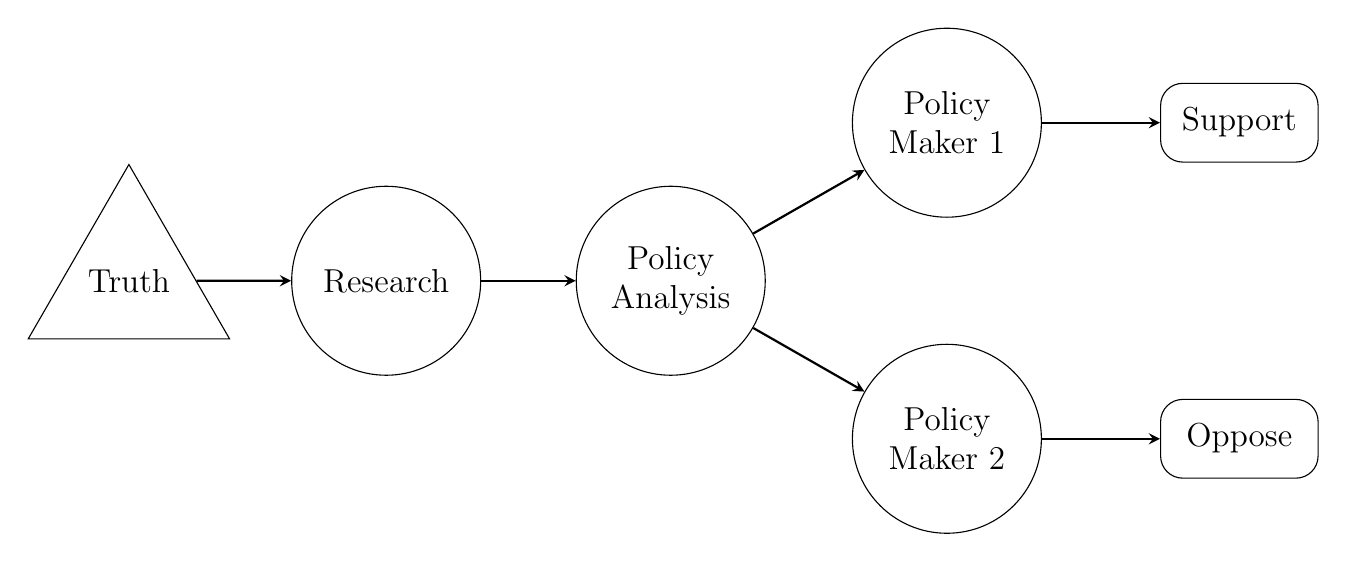
\begin{tikzpicture}[
  every node/.style={font=\large},
  bigcirc/.style={circle, draw, minimum size=2.4cm, align=center, inner sep=2pt},
  tri/.style={regular polygon, regular polygon sides=3, draw,
              minimum size=2.5cm, align=center, inner sep=0pt},
  rrect/.style={rectangle, rounded corners=8pt, draw, minimum width=2cm,
                minimum height=1cm, align=center},
  arr/.style={-stealth, thick}
]

\node[tri]                                        (T)   {Truth};
\node[bigcirc, right=1.2cm of T]                  (R)   {Research};
\node[bigcirc, right=1.2cm of R]                  (PA)  {Policy\\Analysis};
\node[bigcirc, above right=0.3cm and 1.8cm of PA] (PM1) {Policy\\Maker 1};
\node[bigcirc, below right=0.3cm and 1.8cm of PA] (PM2) {Policy\\Maker 2};
\node[rrect,   right=1.5cm of PM1]                (S)   {Support};
\node[rrect,   right=1.5cm of PM2]                (O)   {Oppose};

\draw[arr] (T)   -- (R);
\draw[arr] (R)   -- (PA);
\draw[arr] (PA)  -- (PM1);
\draw[arr] (PA)  -- (PM2);
\draw[arr] (PM1) -- (S);
\draw[arr] (PM2) -- (O);

\end{tikzpicture}
\end{document}
